\documentclass[utf8, 11pt]{feuille}

\newcommand{\titredutd}{\textbf{Devoir maison --- 2022}}

\begin{document}

\begin{center}
Devoir à rendre le mercredi 19 octobre 2022 \\
Chaque étudiant doit rendre son devoir (pas de binôme) manuscrit ou dactylographié
\end{center}

%__________________________________________________________________________________
\section{Défauts de Schottky}

Un type de défaut des cristaux sont les défauts de Schottky où un
atome de l'intérieur migre vers la surface. Le site ainsi libéré s'appelle une lacune.
La formation d'une lacune nécessite de fournir une énergie~$\varepsilon$.
On note: $N$ le nombre d'atomes et~$n$ le nombre de lacunes. Lorsqu'il n'y a pas de lacune,
l'énergie interne du cristal est~$E_0$.

\question
Calculer l'énergie interne~$E$ en fonction de~$E_0$, $n$
et~$\varepsilon$.


\question
Calculer le nombre de micro-états du macro-état à~$n$ lacunes, puis l'entropie~$S(n)$. Pour cela, on considérera que le cristal comporte $N+n$ sites dont $n$ sont inoccupés.

\question Avec l'hypothèse précédente, on inclut les situations où les lacunes sont en surface. Dans ce cas, on ne devrait pas considérer qu'il s'agit de défauts. Expliquer pourquoi dans la limite thermodynamique l'erreur commise sera faible.


\question
Simplifier le résultat de~$S(n)$ en utilisant l'expression approchée
de Stirling du logarithme d'une factorielle.


\question
En déduire la température $T$ en fonction de $n$ et des données.

\question
Exrpimer ~$n$ en fonction de~$T$. Tracer
l'allure de~$n(T)$. Que se passe-t-il à haute température ?


\question
Application numérique: pour le chlorure de sodium il faut~1~eV pour
former une lacune. Calculer la concentration de lacunes à~300~K.


%__________________________________________________________________________________
\section{Cha\^ine de polymères}

Une chaîne comporte $N$ molécules identiques. Chaque molécule peut se trouver dans deux états $\alpha$
ou $\beta$, dont les énergies sont respectivement $\varepsilon$ et 0 (on prend l’énergie de la forme $\beta$ comme référence). Une molécule dans l’état $\alpha$ (resp. $\beta$ ) apporte une contribution $a$ (resp. $b$) à la longueur $L$ de la chaîne. On suppose que l’énergie de la chaîne est fixée et vaut $E$. On suppose que $N \ggg 1$ (il s'agit d'un polymère) et $E \gg \varepsilon$.

\question
Comment varie selon vous $n_{\alpha}$ avec la température $T$ de la chaîne ? Répondre qualitativement mais donner les limites basse et haute température (on précisera par rapport à quoi la température est basse ou haute).

\question
On appelle $n_{\alpha}$ (resp. $n_{\beta}$ ) le nombre de maillons dans l’état $\alpha$ (resp. $\beta$ ). Relier $E$, $\varepsilon$ et $n_{\alpha}$ et $L$ à $a$, $b$, $N$ et $n_{\alpha}$.


\question
Déterminer le nombre d'états microscopiques accessibles $\Omega(E, N)$ de la chaîne isolée. Pourquoi la longueur
$L$ ne figure-t-elle pas comme une variable de $\Omega$ au même titre que le volume intervient dans le cas d’un gaz parfait ?



\question
Déterminer l'entropie puis la température $T$ en fonction de N et de $n_{\alpha}$. En déduire $n_{\alpha}$, puis $E$ en fonction de $N$ et $T$. En déduire la capacité calorifique de la chaîne et tracer là sommairement en fonction de $T$.

\question Quelle est, en fonction de $T$ et $\varepsilon$, la fraction de molécules $f_{\alpha}$ dans l’état $\alpha$ ? Simplifier cette expression dans la limite des hautes et basses températures.

\question
Montrer que $S/(N k_B) = - f_{\alpha} \ln f_{\alpha} - f_{\beta} \ln f_{\beta}$. Interpréter cette identité. Existe-t-il une identité similaire pour un gaz parfait ?





%__________________________________________________________________________________
\section{Question de contact thermique}
En étudiant un système à deux niveaux, nous avons obtenu la température micro-canonique pour les spins nucléaires d'un cristal associée à l'énergie magnétique $E_m$, que nous noterons $T_m(E_m)$. Des inversions de population correspondant à des températures négatives ont été observées dans un cristal de fluorure de lithium. Dans ce système, le temps de relaxation pour l'interaction mutuelle entre les spins nucléaires ($\tau_1 \simeq 10^{-5}$ s) est très court devant le temps de relaxation pour l'interaction entre les spins et le réseau ($\tau_1 \simeq 3 \times 10^{2}$ s). On peut donc rapidement arriver (sur une échelle $\tau_1$) \`a un équilibre thermodynamique du système de spins nucléaires avant que ce système ne se thermalise avec les vibrations du réseau. L'expérience consiste alors à placer le cristal dans un champ magnétique et à renverser très brutalement celui-ci. On est alors, pendant un temps de l'ordre de $\tau_2$ dans un état de température négative (voir figure ci-dessous).

\begin{figure}[!t]
\centering
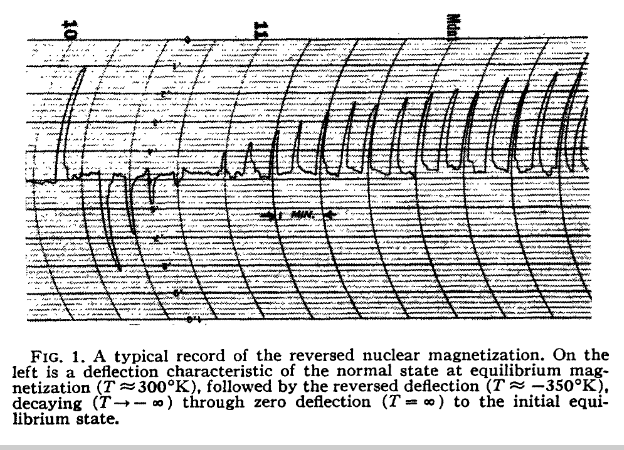
\includegraphics[height=.38 \textwidth]{negative}
\caption{Extrait de l'article : E. M. Purcell and R. V. Pound, Physical Review \textbf{81}, 'A nuclear spin system at negative temperature', p. 279 (1951)}
\label{FTN}
\end{figure}

On considère donc $N$ atomes d'un cristal qui portent chacun un spin-1/2, juste après l'inversion du champ magnétique $B$ qui les avait polarisés. L'énergie magnétique $E_m^i$ est donc positive. Par ailleurs, pour tenir compte les vibrations du cristal, on admet que ces $N$ atomes  portent des oscillateurs harmoniques classiques indépendants 3D (masse $m$, pulsation $\omega$). L'énergie vibrationnelle initiale est notée $E_v^i$.


\question
Rappeler les expressions $S_v(E_v^i,N)$ , $T_v^i$, $S_m(E_m^i,N)$ et $T_m^i$ des entropies et des températures en fonction des données, de $N$, et des énergies initiales.


\question
Mener l'étude du contact thermique entre les degrés de liberté de spins et vibrationnels. Le résultat n'est pas analytique. On déterminera l'équation qui permet de calculer l'énergie magnétique la plus probable, que l'on assimilera à l'énergie magnétique à l'équilibre. Préciser la température d'équilibre $T^f$ que l'on comparera à $T^i_v$ et $T_m^i$.


\question
Décrire thermodynamiquement la transformation du système. Justifier que les températures négatives sont plus chaudes que les températures positives.




\end{document}
